% Deve resumir o experimento, os resultados e a discussão (comentários)
% e incluir opiniões do grupo e propostas futuras para o experimento
%Descrição do hardware
%Descrição do software
%\cite{Advpdf}
%\cite{thepdf}
%\cite{dsl}
Na seção desenvolvimento deve ser respondidas as seguintes perguntas:
 
	\begin{itemize}
		\item Estrutura do Programa: Qual a estruturação/arquitetura do Programa?
	 	\item Qual é o procedimento para a execução do programa? 
	 	\item Quais artefatos são necessários para a execução do programa?
	 	\item Quais os problemas técnicos enfrentados no desenvolvimento do programa?
	 	\item Como os pontos relacionados à disciplina foram abordados no problema? Quais as lições aprendidas? Quais as principais dificuldades?
	 	\item Quais elementos teóricos abordado na disciplina foram implementados no programa?
	 	\item Quais adaptações, extensões, bibliotecas externas, foram necessários para a solução do problema?
	 	\item Caso use parte de códigos disponibilizados na Web, colocar referência \footnote{A home-page de onde tirei
este material:\url{http://en.wikibooks.org/wiki/LaTeX}.Estou formatando para \LaTeX apenas para os estudantes irem se orientando de como e o quê escrever.Assim, me isento de responsabilidade sobre o conteúdo deste texto. Dúvidas: carla(rocha.carla@gmail.com)}
	\end{itemize}
	
	As Figuras são simplesmente inseridas como mostrado na Fig. \ref{Fig1}
	
\begin{figure}[ht]
  \centering
  %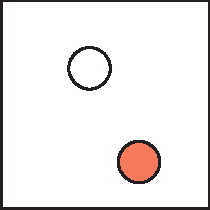
\includegraphics[width=5cm]{figs/samplefigure}
   \caption{Arquitetura do Programa.}
  \label{Fig1}
\end{figure}
 
\subsection{Artefatos}
\label{SebSec:Artefatos}
Os artefatos entregues devem ser documentados no relatório:
\begin{itemize}
\item Arquivos contidos no programa. Lista dos nomes dos arquivos, assim como a extensão dos arquivo
\item Aquivo README, com instruções de uso do software desenvolvido e necessidades técnicas para a execução do programa
\item Arquivos de entrada/saída, caso necessário.
\end{itemize}

